\chapter{Analyse, fortolkning og resultater}
\label{Ch:4}

I det følgende afsnit betragtes den empiri som er indsamlet i forbindelse med dette projekt.  I afsnit \vref{sec:spø} betragtes den empiri som er indsamlet gennem det første spørgeskema, i afsnit \vref{sec:sam} gennemgåes den indsamlede empiri fra spørgeskema to, og kapitlet afsluttes med et afsnit \vref{sec:afv} hvor forskellige elevers skriftlige arbejde analyseres vha. TAP modellen.

\section{Spørgeskemaet}
\label{sec:spø}
Som empirisk grundlag for dette projekt er der indsamlet data via et spørgeskemaer samt fra elev afleveringer i to forskellige klasser. Besvarelserne, fra 1.g elever på Viborg Katedralskole, på spørgeskemaet er indsamlet med SurveyXact, der har været 117 besvarelser ud af 349 mulige besvarelser hvilket giver spørgeskemaet en svarprocent på \mbox{33,5 \%}. Undersøgelsen er blevet gennemført i forbindelse med praktisk eksperimentelt arbejde, hvor eleverne har besværet de fem spørgsmål umiddelbart efter det eksperimentelle arbejde og umiddelbart forud for det skriftlige arbejde. De 117 svar fordeler sig som vist på figur \vref{fig:4.1.a}. 

\begin{figure}[h!]
	\centering
	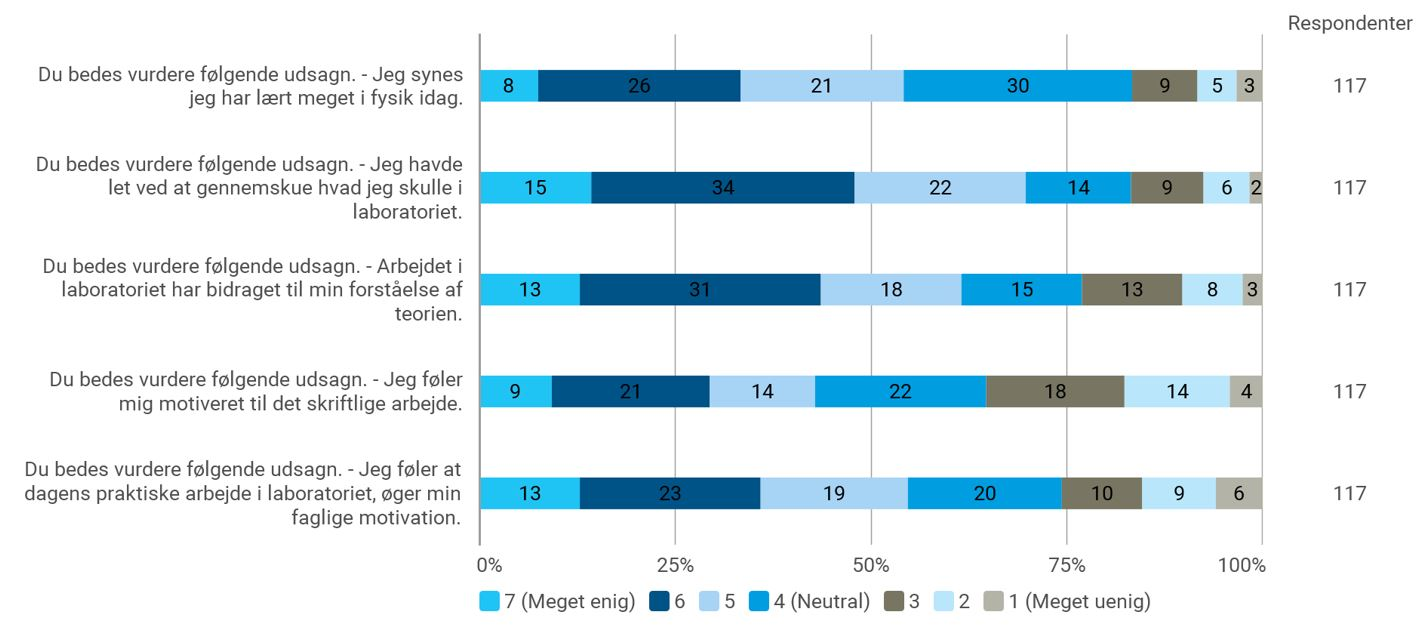
\includegraphics[width=0.9\textwidth]{Figs/Sammenlign}
	\caption{Det samlede datasæt for de fem spørgsmål med hver 117 respondenter fra en 1.g årgang på Viborg Katedralskole. Svar procenten for undersøgelsen er på omkring 33 \%. }
	\label{fig:4.1.a}
\end{figure}
Betragter man antallet af positive svar på de fem udsagn, hvor et svar regnes som positivt hvis der er svaret fire eller højere. Så vil gennemsnitet af besvarelserne være 66,32 \% af de afgivne svar i alle fem spørgsmål.  Hertil kunne det anfægtes om eleverne faktisk har forstået hvad de har svaret på. Her ville man ved hjælp af Cronbach's $\alpha$ kunne afgøre om der er en intern konsistens i de afgivne svar.

\subsection*{Chronbach $\alpha$}
\begin{table}[h!]
	\centering
	\caption{Her ses værdier for Cronbach's $\alpha$ som mål for at teste den interne konsistens i undersøgelsen. Data som disse kan findes i en lang række artikler, men her følger vi udlægningen af \citep[Tabel 1, s. 382]{Peterson1994} hvor der er en række forskellige fortolkninger, den her anvendte tager sit udgangspunkt her og er så tilpasset.}
	\label{tbl:alpha}
	\begin{tabular}{@{ } c c @{ }}
		\toprule[2.pt]
		Værdi af Cronbach's $\alpha$ & Intern konsistens\\
		\midrule
		$0.9\leq \alpha$ 		& Fremragende\\
		$0.8\leq \alpha < 0.9$ 	& God\\
		$0.7\leq \alpha < 0.8$	& Acceptabel\\
		$0.6\leq \alpha < 0.5$	& Tvivlsom\\
		$0.5\leq \alpha < 0.6$ 	& Dårlig\\
		$\alpha < 0.5$			& Uacceptabel\\
		\bottomrule[2pt]
	\end{tabular}
\end{table}
Cronbach's  $\alpha$ er beregnet på følgende vis: 
\begin{equation}\label{eq:alpha}
	\alpha = \left(\frac{k}{k-1}\right)\cdot \left(1-\sum_{i=1}^{k} \frac{\sigma^{2}_{i}}{\sigma^{2}{s}}\right)
\end{equation}
hvor $k$ er altallet af målinger i undersøgelsen, $\sigma^{2}_{i}$ er variansen af den i'te måling, mens $\sigma^{2}_{s}$ er variansen for hele undersøgelsen, jf \cite[s.382]{Peterson1994}. For de indsamlede data i spørgeskemaet er Cronbach's $\alpha$ beregnet til 0.91, hvilket baseret på skalaen i tabel \vref{tbl:alpha} betyder at der er en fremragende intern konsistens i undersøgelsen. Hvilket igen betyder at elevernes svar er konsistente gennem alle spørgsmålene. 

På baggrund af de 117 besvarelser af spørgeskemaet er det muligt at beregne en Chronbach $\alpha$ for datasættet. Her findes værdien for Chronbach $\alpha$ til 0,91 hvilket tyder på at der er en virkelig god intern konsistens i undersøgelsen jf. tabel \tbref{alpha}. Det tyder også på at eleverne har forstået de fem spørgsmål som de er blevet bedt om at svarer på.  Generelt ser det ud til at hvis en elev svarer lavt, kategori 1 og 2, på spørgsmål et så svarer den pågældende elev lavt på alle fem spørgsmål. Ligeledes hvis en elev svarer højt, kategori 6 og 7, så svarer de generelt over middel på alle spørgsmålene.

\subsection*{Opsamling på spørgeskemaet}
Det er altså tydeligt med udgangspunkt i den empiri der er indsamlet i forbindelse med spørgeskema undersøgelsen at eleverne generelt føler at de lære noget af det praktiske arbejd, samt at de kan gennemskue hvad de skal i laboratoriet, men det halter stadig med at kunne motivere eleverne til det skriftlige arbejde, som det fremgår af figur \firef{4.1.a}.
Kigger man på nogle af de kommentarer som eleverne har givet finder man udsag som:
\begin{quote}
	``\emph{Jeg har i dette forløb om ideal gasser, været lidt udfordret pga at vi ikke har fået noget teori forklaret på tavlen. Dette gjorde mig en del umotiveret.}''
\end{quote}
Dette til trods for at den pågældende elev har vurderet alle fem spørgsmål højt eller meget højt. Så der er en klar udfordring i hvorledes resultaterne så skal fortolkes, når eleverne vurderer udsagnene på en måde og efterfølgende skriver noget anden end det deres vurdering umiddelbart ser ud til. Det er dog tydeligt at denne pågældende elev er udfordret af \ib{}-tilgangen til undervisningen.
En af de store udfordringer i forbindelse med denne undersøgelse er at det ikke er muligt at trække de elever ud som har været i test gruppen og se på deres resultater uafhængigt af de øvrige 1.g elever, da spørgeskemaet har været gennemført anonymt for at opnå så pålidelige og reelle svar fra eleverene. Det er dermed kun muligt at hente information om eleverne er en del af test gruppen såfremt de som i udsagnet ovenfor klart giver udtryk for at de tilhører testgruppen. den overordnede konklusion ser ud til at være at eleverne generelt motiveres ved at lave eksperimenter i fysikfaget men at det halter med at motivere eleverne til det skriftlige arbejde i fysikfaget.  

\section{Samtale om motivation for skriftlighed}
\label{sec:sam}


\section{Afleveringer}
\label{sec:afv}
Til at belyse den anden del af denne undersøgelse nemlig spørgsmålet om hvorvidt den skriftlige kompetence udvikles gennem anvendelsen af \ib{} og SWH i samspil. Anvendes elev afleveringer, som analyseres efter Toulmins Argumentations Princip (TAP). I denne del af empirien analyseres fire afleveringer fra klassen 1.y hvor der udtages to tilfældigt valgte afleveringer fra den første rapport som eleverne afleverede og to fra den aflevering eleverne afleverede lige inden påske. På samme vis er der udtaget to gange to afleveringer fra en anden 1.g klasse på Viborg Katedralskole.
De otte afleveringer er fordelt på følgende måde hvor elev 1 og elev 2 er fra kontrolgruppen: 
\begin{enumerate}
	\item[Elev 1] 1.e - Nyttevirkning af elkedel og kaffemaskine samt Bestemmelse af bølgelængde for laserlys\vspace{-15pt}
	\item[Elev 2] 1.e - Nyttevirkning af elkedel og kaffemaskine samt Bestemmelse af bølgelængde for laserlys\vspace{-15pt}
	\item[Elev 3] 1.y - Undersøgelse af fænomenet gnidning og Undersøgelse fænomenet diffraktion\vspace{-15pt}
	\item[Elev 4] 1.y - Undersøgelse af fænomenet gnidning og Undersøgelse fænomenet diffraktion
\end{enumerate}
 \subsection*{Nyttevirkning af elkedel og kaffemaskine}
Når man ser på de første to rapporter fra hhv. elev 1 og elev 2 så er det svært at indetificere det skema som er beskrevet på figur \firef{tou}. Der er i høj grad tale om en rapport som er skrevet med ført hånd af den vejledning som eleverne har fået på forhånd. Det har været helt klart for eleverne hvilket resultat de forventedes at opnå med øvelsen. Det tætteste vi kommer på en egentlig påstand er følgende pasus
\begin{quote}
	``\emph{$\Delta$Enytte er den energi, som udnyttes til opvarmning af vandet. Når vi har en mængde vand med massen m, kan denne energi beregnes ved hjælp af formlen;
	\begin{equation*}
	\Delta Enytte = m\cdot c\cdot \Delta T
	\end{equation*}
	hvor $c$ er den specifikke varmekapacitet (varmefylde) for vandet.}''
\end{quote}
Problemet her er at denne påstand ikke er funderet i data så det er i virkeligheden det facit som eleven burde nå frem til men hvordan undersøges dette? det er temmelig uklart for undertegnede. For både elev 1 og elev 2 er data her forstået som tal tastet ind i et skema som har været tegnet op på forhånd. Eleverne har dermed blot skulle taste tydeligt definerede værdier ind i skemaet, i passende allerede angivne enheder. Data er for de to grupper ikke overraskende meget lig hinanden. I forhold til at skabe evidens for den påstand som famgår af tekstuddraget her over, så forbliver evidensen her blot udregninger med de allerede givne formler. Sluttelig er rygdækningen her den første del af rapporten hvori teorien gennemgåes, dog med det lille aberdaby at dette afsnit mere eller mindre kommer fra øvelsesvejledningen.
